% Created 2019-11-29 Fri 10:30
% Intended LaTeX compiler: pdflatex
\documentclass[11pt]{article}
\usepackage[utf8]{inputenc}
\usepackage[T1]{fontenc}
\usepackage{graphicx}
\usepackage{grffile}
\usepackage{longtable}
\usepackage{wrapfig}
\usepackage{rotating}
\usepackage[normalem]{ulem}
\usepackage{amsmath}
\usepackage{textcomp}
\usepackage{amssymb}
\usepackage{capt-of}
\usepackage{hyperref}
\author{Tigany Zarrouk\thanks{tigany.zarrouk@skf.com}}
\date{25.11.2019}
\title{Dislocation mediated C migration in Fe Dark Etching Regions}
\hypersetup{
 pdfauthor={Tigany Zarrouk},
 pdftitle={Dislocation mediated C migration in Fe Dark Etching Regions},
 pdfkeywords={},
 pdfsubject={},
 pdfcreator={Emacs 26.3 (Org mode 9.1.9)}, 
 pdflang={English}}
\begin{document}

\maketitle


\section*{Motivation}
\label{sec:orga348fc6}
\begin{itemize}
\item Rolling contact on bearing raceways generate maximal shear
stresses in subsurface.
\item Degradation in subsurface microstructure observed due to
plasticity.
\item This can lead to failure by Rolling Contact Fatigue (RCF).
\item Degradation arises in form of Dark Etching Regions (DERs),
characterised by development of ferrite features with patches of
unaltered martensitic matrix.
\item Carbon redistribution is thought to be a fundamental mechanism
behind DER formation.
\item Dislocation-driven carbon migration has been suggested but hard to
experimentally verify.
\item Atomistic modelling necessary to ascertain if dislocations move
carbon and the underlying mechanism.
\end{itemize}

\section*{Aims}
\label{sec:org74b04da}
To answer the questions:
\begin{itemize}
\item Do dislocations move carbon?
\item Do temper carbides dissolve/grow with rolling contact fatigue?
\end{itemize}



\section*{Objectives}
\label{sec:org7649f73}

\begin{itemize}
\item Build Kinetic Monte-Carlo model of dislocation motion.
\item Tight-binding used to obtain formation energies:
\begin{enumerate}
\item Kink-pair formation energies as a function of carbon content
and stress.
\item Dissolution energies of carbon near core of dislocation as a
function of stress.
\end{enumerate}
\end{itemize}


\section*{Methods}
\label{sec:org6d43c5f}
\begin{itemize}
\item Density Functional Theory is not feasible.
\item Use tight-binding: rigorous approximation to DFT.

\item Boundaries of cell affect relaxation of core more.
\item Semi-empirical method is more computationally efficient.
\end{itemize}



\subsection*{Tight Binding}
\label{sec:orge1212fd}


\begin{itemize}
\item Tight binding is an approximation to DFT.
\item Overlaps between atomic orbitals are key parameters.
\item Parameters can be fitted to experimental data
\item \(\mathcal{O}(N^3)\), but much smaller prefactor compared to DFT.
\end{itemize}

\subsection*{BOP}
\label{sec:org810310a}

\begin{itemize}
\item BOP is a faster but less accurate \(\mathcal{O}(N)\) method of interatomic
force calculation within tight-binding.
\item One builds a local density of states from moments, giving detailed
electronic structure information.
\end{itemize}


\subsection*{Embedding}
\label{sec:orgae8e992}

\begin{itemize}
\item Idea is to combine speed of BOP (\(\mathcal{O}(N)\)) with accuracy of
tight-binding \(\mathcal{O}(N^3)\).
\item Increasing the number of atoms gives freedom to:
\begin{itemize}
\item Investigate isolated dislocations.
\item Include solutes at more realistic concentrations.
\item Simulate interfaces near a surface (e.g. TiO\(_2\) and
bulk Ti)
\end{itemize}
\end{itemize}
\begin{NOTES}
Invariance theorem with green's function approaches. So good with boundary
conditions. 
\end{NOTES}

\section*{Defect Clusters}
\label{sec:orgec2ee65}

\begin{itemize}
\item Increase in oxygen content in Ti-7wt.\%Al causes higher number density of
\(\alpha_2\) precipitates at 550\textdegree{} C (Felicity's results).
\item Oxygen acting as a defactant might stabilise defect complexes (Ti\(_{\text{v}}\) + nO).
\item This can cause more defects resulting in the increased number of precipitates due to more nucleation sites.
\item First starting out with pure Ti and \(\alpha_2\). Still working on extension to Ti-7wt.\%Al.
\end{itemize}


\subsection*{Calculation Details}
\label{sec:org7c88fdb}
\begin{itemize}
\item Först \emph{et al.} \([3]\) calculated energetics of defect complexes with associated local
force-constant matrix.
\item Partial thermodynamic equilibrium imposed (thermal equilibrium for one species and not the other).
\item Defect concentration plotted as a function of carbon/vacancy concentration
only at 160\textdegree{} C.
\item Extension: apply the quasiharmonic approximation/do thermodynamic integration
for better accuracy at higher temperatures (550\textdegree{} C - 950\textdegree{} C).
\end{itemize}

\([3]\) \emph{Point Defect Concentrations in Metastable Fe-C Alloys}, Först \emph{et
al}, Phys. Rev. Lett. 96, 2006



\subsection*{Plots in Fe-C}
\label{sec:orgee3b694}
\begin{center}
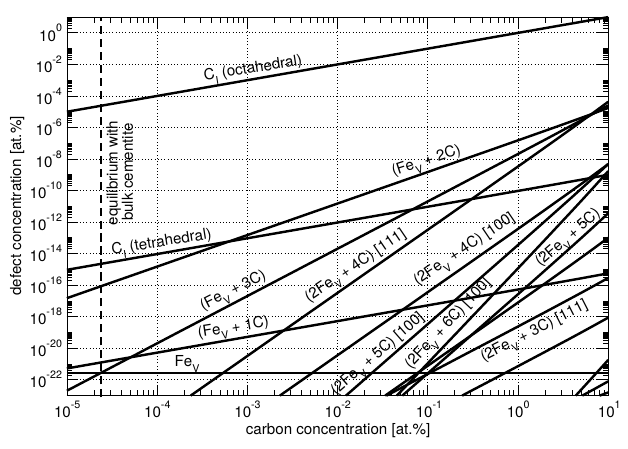
\includegraphics[width=.9\linewidth]{/home/tigany/Documents/docs/Management/Images/forst_defect_concentration_cementite.png}
\label{org9f5fd4a}
\end{center}

\begin{center}
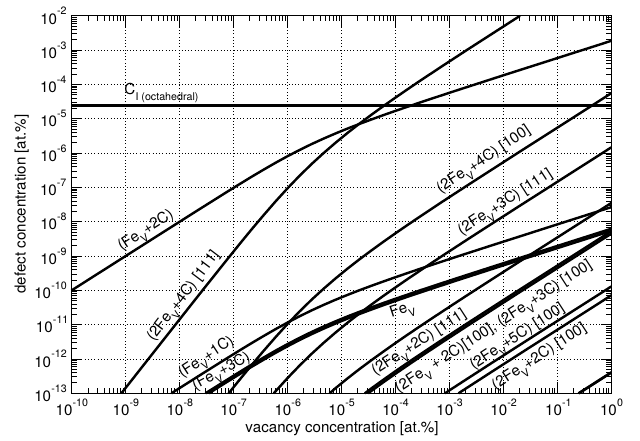
\includegraphics[width=.9\linewidth]{/home/tigany/Documents/docs/Management/Images/forst_defect_concentration_vacancies.png}
\label{orgff7425a}
\end{center}

\subsection*{\(\text{Ti}_{3}\text{Al}\)  Cells}
\label{sec:org42d2e7e}
\begin{center}
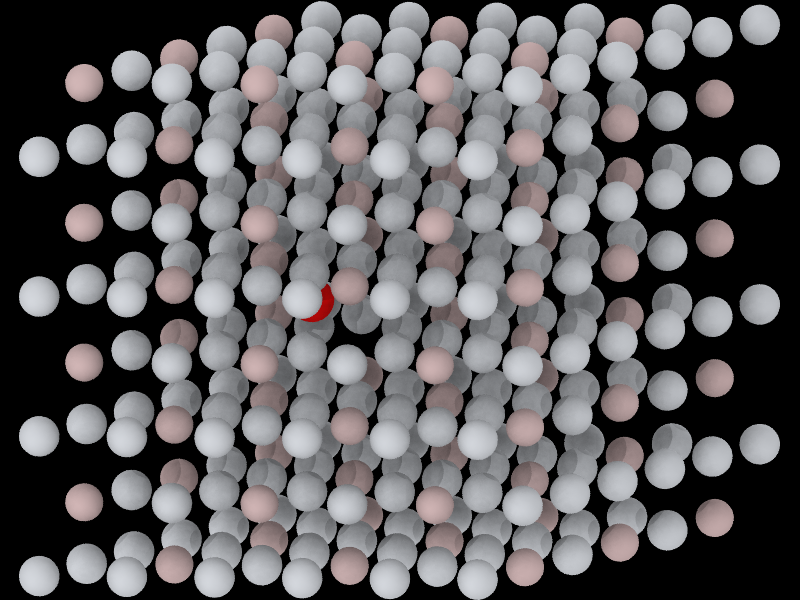
\includegraphics[width=.9\linewidth]{/home/tigany/Documents/docs/Management/Images/ti3al_val_o.png}
\label{org04ceecc}
\end{center}

\subsection*{Ti Cells}
\label{sec:orgad3a9ad}


\subsection*{Defect Clusters: Future Work}
\label{sec:org959d9ae}
\begin{itemize}
\item Finish Ti and \(\text{Ti}_{3}\text{Al}\) defect cluster calculations in DFT.
\item Possibly extend to Ti-7wt\%Al with SQS structures.
\item See how much of an effect anharmonicity has on predictions.
\end{itemize}


\section*{Summary}
\label{sec:orgcf3bd41}
\begin{itemize}
\item Successfully made TB model of Ti which reproduces DFT results with only
d-orbitals.
\item Transferable:
\begin{itemize}
\item Correct energetic ordering for study of different phases.
\item Correct elastic properties and good scaling for defect simulations.
\item Integer number of electrons for charge transfer models (electrochemistry).
\end{itemize}
\item BOP formulation produces similar results with only linear scaling.
\item Embedding calculations should resolve single dislocation core ground-state
at realistic O concentrations.
\item To do: Embed O-disl, \(\text{Ti/TiO}_2\) interface, defect clusters.
\end{itemize}
\end{document}